%!TEX root = /Users/zolkko/Projects/zolkko-alarm/doc/main.tex
\subsection{Разработка печатной платы управляющего устройства в Eagle}
Запуск редактора топологической схемы с системе Eagle PCB осуществляется в Ealge Layout Editor
нажатием кнопки ''Board''.  При этом, в выведенном на экран редакторе топологических
схем (рис. \ref{img:boardEd}), будут размещены корпуса всех используемых на принципиальной
электрической схеме компонентов. 

\begin{figure}[h]
	\center{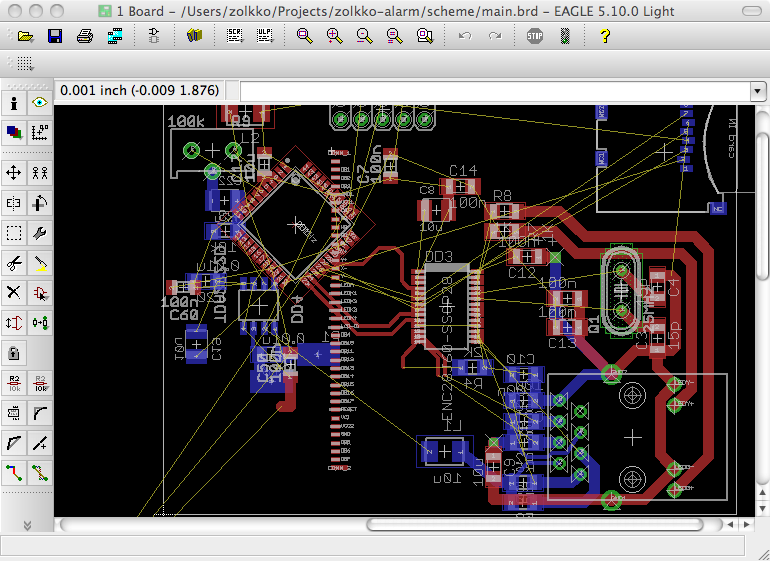
\includegraphics[bb=0 0 770 561, clip, scale=0.5]{board_ed.png}}
	\caption{Окно редактора топологических схем системы Eagle}
	\label{img:boardEd}
\end{figure}

Перед тем как начать фактическое создание печатной платы, необходимо произвести
первоначальную настройку рабочего окружения редактора печатных плат. А именно, необходимо
включить поддержку векторных шрифтов. Так как если это не сделать, то любой введённый текст в
слое ''silkscreen'' не будет отображаться.

Следующий подготовительный этап -- корректировка границ печатной платы. По умолчанию граница
печатной платы в Eagle имеет смещение в 0.1 дюйм. Для корректировки положения
нижнего левого угла печатной платы нужно в диалоговом окне задания свойств бордюра
печатной платы задать значение смещения в 0.0 дюйма.

После этого необходимо скорректировать размер самой печатной платы. В
бесплатно распространяемой версии Eagle имеется ограничение по максимальному размеру
печатной платы. Однако, проектируемое мной <<универсальное устройство управления
температурой на базе микроконтроллера AVR семейства XMega>> подходит под эти ограничения.

\subsubsection{Размещение компонентов на печатной плате}
На этом этапе производится размещение компонентов на плате. Так как в
бесплатно распространяемой версия системы Eagle отсутствует функция автоматической
расстановки компонентов на печатной плате, то выполнить это действие необходимо в ручную,
перенося компоненты в область печатной платы. При этом необходимо самостоятельно
контролировать некоторые аспекты проектирования, а именно как можно ближе располагать
фильтры по линиям питания с корпусами микросхем, согласование расположения разъёмов с
корпусом проектируемого устройства.

Следующим этапом является размещение монтажных отверстий на печатной плате.
Расстановка монтажный отверстий производится при помощи инструмента ''Drill Holes''. Для того,
чтобы сконфигурировать размер отверстия и его окантовки  нужно вызвать диалог ''свойства''
этого монтажного отверстия и в комбинированном выпадающем списке задать необходимый размер.

\subsubsection{Трассировка печатной платы}
После того, как все компоненты, монтажные отверстия размещены на печатной плате и
сконфигурированы геометрические параметры самой печатной платы, необходимо произвести
трассировку печатной платы.

Сигнальные линии, соединяющие компоненты в редакторе  топологических схем системы Eagle,
отображаются в виде линий жёлтого цвета. Для того, чтобы редактор обновил их расположение
и нашёл наиболее кратчайший путь, нужно  выполнить команду ''Rateness''.

Редактор топологических схем системы Eagle позволяет производить разводку печатных плат в
двух режимах: ручном и автоматическом.

В случае если сигналы в проектируемом устройстве не критичны к сопротивлению проводящих
трасс и не предъявлется специальных требований к их частотным характеристикам,- для разводки
печатной платы можно использовать инструмент ''Autorouter''  -- автоматически разводящий все
сигналы на проектируемой печатной плате.

Перед проведением трассировки печатной платы необходимо задать параметры контроля
геометрических требований проекта (DRC). Для этого необходимо вызвать команду ''Design Rules''
главного меню ''Edit'' редактора топологических схем, так же необходимо задать параметр
размерности сетки редактора. Задание этих параметров повышает качество автоматической
трассировки и избавляет от необходимости ручной корректировки результатов трассировки.

Для выполнения автоматической трассировки платы нужно выполнить команду ''Auto''. Вызов
этой команды приведёт к отображению диалогового окна задания параметров трассировки.

Для получениея приемлемого результата при трассировке разрабатываемой печатной платы
в диалоговом окне ''Autorouter Setup'' мной был задан параметр сетрки трассировки в значении
равном значению размерности сетки редактора.

Диалоговое окно настройки параметров ''Autorouter Setup'' позволяет сохранять и загружать
конфигурационные файлы настройки трассировки.

После установки всех необходимых параметров трассировки необходимо нажать на кнопку
''Ok'', что приведёк к фактическому запуску встроенной программы--трассировщика.

В системе Eagle так же возможно использовать внешнюю программу трассировки.
Для этого необходимо воспользоваться встроенным CAM процессором системы для
преобразования файлов формата ''brd'' в файлы ''dsn'', используемых в большинстве
программ--трассировщиках. Результат работы внешнего трассировщика необходимо
импортировать в систему Eagle, используя обратное преобразование.

\subsubsection{Создание заливки в редакторе топологических схем системы Eagle}
Заливка -- медный слой (copper pour, copper plane), часто используемый для создания
слоёв экранирования. Так же применяется для уменьшения количества меди, которую
необходимо удалять с заготовки в процессе создания печатной платы.

Для создания заливки в редакторе топологических схем системы Eagle существует
инструмент Polygon.

Выбрав этот инструмент, необходимо очертить полигон подлежащий заливке. После чего
назначить ему имя сигнала, для которого будет создаваться заливка. Для задания имени
полигона необходимо:
\begin{itemize}
	\item{} выбрать инструмент ''Name'';
	\item{} выбрать целевой полигон;
	\item{} в отображённом диалоговом окне ввести наименование сигнала;
	\item{} завершить задание имени нажатием кнопки ''Ok''.
\end{itemize}
Для того, что бы созданная заливка не пересекалась с другими сигналами на печатной
плате необходимо задать параметры ''Isolate'' и ''Spacing'' полигона заливки. Задание
этих параметров производится в диалоговом окне ''Properties''
полигона (рис. \ref{img:polyProperty}). В этом же диалоговом окне можно задать требуемый вид
заливки: сплошной или сетчатый.
\begin{figure}[h]
	\center{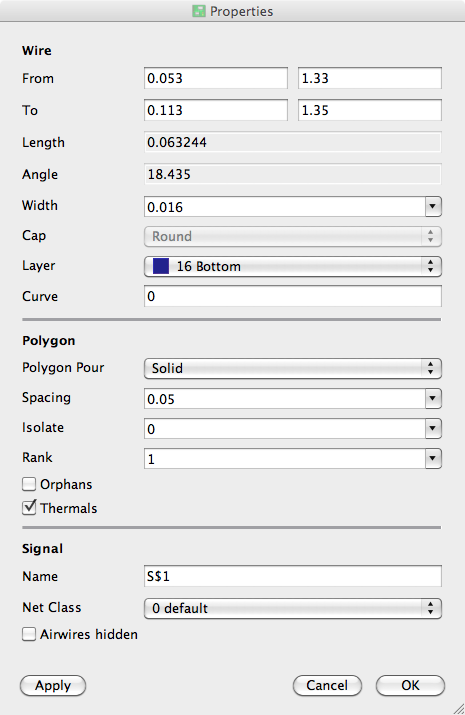
\includegraphics[bb=0 0 465 715, clip, scale=0.4]{polygon_property.png}}
	\caption{Диалоговое окно ''Properties'' полигона системы Eagle}
	\label{img:polyProperty}
\end{figure}


Результатом проделаной работы стала схема топологическая (приложение В).
